% This example An LaTeX document showing how to use the l3proj class to
% write your report. Use pdflatex and bibtex to process the file, creating
% a PDF file as output (there is no need to use dvips when using pdflatex).


\documentclass{l3proj}

\begin{document}

\title{Global Rugby Network FanZone (Web)}

\author{Ruxandra Bob \\
		Marios Constantinou \\
        Daniel Juranec \\
        Arnas Kapustinskas \\
        Andrew McCluskey}

\date{10 February 2017}

\maketitle

\begin{abstract}

The abstract goes here

\end{abstract}

%% Comment out this line if you do not wish to give consent for your
%% work to be distributed in electronic format.
\educationalconsent

\newpage

%==============================================================================
\section{Introduction}

Software engineering

This paper presents a case study of...


%% Final paragraph.
The rest of the case study is structured as follows.  Section
\ref{sec:background} presents the background of the case study
discussed, describing the customer and project context, aims and
objectives and project state at the time of writing.  Sections
\ref{sec:alice} through Section \ref{sec:managing} discuss issues that
arose during the project...

%==============================================================================
\section{Case Study Background}
\label{sec:background}

Include details of

\begin{itemize}
\item The customer organisation and background.
\item The rationale and initial objectives for the project.
\item The final software was delivered for the customer.
\end{itemize}

%==============================================================================
%\section{Alice}
%\label{sec:alice}
%\begin{figure}
\begin{center}

\includegraphics[width=7cm]{figures/alice}
\end{center}
\caption{Behind it was a little door}
\label{fig:alice}
\end{figure}
%==============================================================================
\section{Continuous Integration and Continuous Deployment Considerations}
\label{sec:CICD}

The project used a multitude of Continuous Integration (CI) and Continuous
 Deployment (sometimes Delivery) (CD) techniques. A CI server's purpose "is to check the code
 repository for changes, check out the code if it spots any, and run a
 list of commands to trigger the build."\cite{meyer2014continuous} A build is "ideally more than just
 compiling—it should also include a thorough test suite to help verify that the code
 still works with every change."\cite{meyer2014continuous} This gives a development
 team a quick, automated way of checking their code works, follows a style guide and
 doesn't break any other work. 
 
One of the key concepts of CI is often phrased as: "Commit Daily, 
 Commit Often"\cite{meyer2014continuous}. For our project, this was sometimes a struggle. 
 This was due to a small number of factors, which boiled down to: "We don't work on the project 
 every day", and "I'm not used to git". There was little we could do to remedy the former issue - 
 all we could do was commit often \textit{whilst we worked on the project}. The gitflow 
 branching system we used in the VCS (see section \ref{sec:VCS}) was unfamiliar to several 
 members of the team, and it took time for everyone to become accustomed to the system. As the
 project progressed however, more builds were made, more commits pushed, and more bugs found.

Another hurdle at which we fell was getting into the habit of writing tests for our code. I shall 
 mention this briefly here, but for more details please see section \ref{sec:testing}. In Fowler's 
 2006 paper on CI, he says: "Imperfect tests, run frequently, are much better than perfect tests 
 that are never written at all."\cite{fowler2006continuous}
 
 %TODO: COVERAGE PICTURE

Continuous Deployment is the practice of continually deploying working builds to production
 as often as possible. It adheres to the Agile principles of:
 \begin{itemize}
 \item
 Our highest priority is to satisfy the customer
 through early and continuous delivery
 of valuable software. \cite{agileprinciples}
 \item 
 Deliver working software frequently, from a 
 couple of weeks to a couple of months, with a 
 preference to the shorter timescale. \cite{agileprinciples}
 \end{itemize}
 In our project, as soon as a new feature is merged into the dev branch,
 tests are run, and then the changes are deployed to a staging server, hosted by firebase. Similarly,
 as soon as dev is merged into master, master is pushed to our production server, also hosted by firebase.
 The dev branch was typically merged into master once a week, allowing time for any changes to be made 
 to features that weren't quite perfect, and to iron out any bugs that were found after time in dev.
 
Our CI and CD was operated using Gitlab's integrated CI system. This uses docker to
 run a set of instructions defined in the 'gitlab-ci.yml' file.  Instructions are 
 separated into tasks. Tasks belong to stages - in our project, these were
 "test" and "deploy". The tasks are run as builds within a pipeline. The docker instances were
 in some cases hosted for free by Gitlab (sponsored by a cloud company). In other cases,
 builds were run on team computers. A common upper limit for build time is quoted as 
 10 minutes\cite{fowler2006continuous} - ours typically ranged from 5-15 minutes, with some exceptions that were 
 typically waiting on the gitlab CI runners to free up. The single largest time-drain was
 running \texttt{npm install} every time docker span up a new instance. Running tests typically took under
 a minute after this.
 
 %TODO: Times Figure
 \begin{figure}[H]
\begin{center}
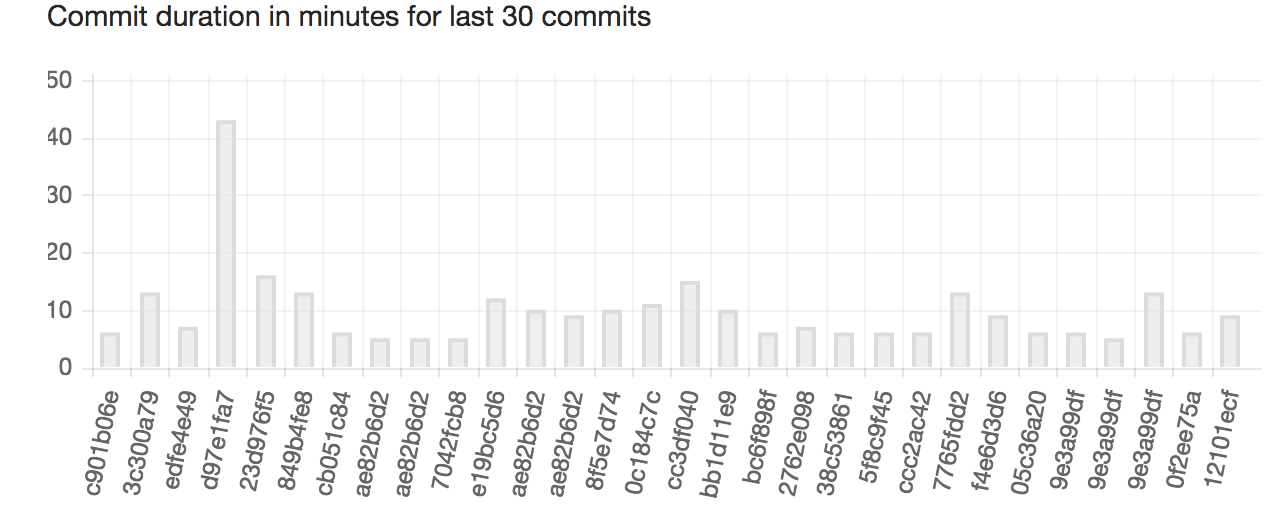
\includegraphics[width=9cm]{figures/cicd_build_duration}
\end{center}
\caption{Build Duration for last 30 commits from 21:28 on 19/03/2017}
\label{fig:cicd_build_duration}
\end{figure}



% Describe Linting task
The first task used by the project's 'test' stage ran a series of lint checks over the 
 project's source code. Linting involves performing static analysis on code to detect bugs 
 or violations of a style guide. These kind of checks are also performed by compilers and 
 so on. These issues can range from missing semicolons, to using a mix of 
 double and single quotes, to whether a function is never called. The task tested CSS, 
 JSON, typescript, javascript,  HTML and LESS. Whilst this was often annoying, these tests 
 did help maintain a higher quality of code in the codebase. As our policy was to not allow a 
 merge to dev take place if a branch was not passing tests, we had a method of 
 enforcing that the standards we defined were upheld.

% Describe testing task
The second task ran the project's tests. Again, this task had to complete successfully in 
 order for a branch to be merged into dev. This stage also generated coverage reports which 
 were used to give the team an indication of how well our code was tested.
 
 \begin{figure}[H]
\begin{center}
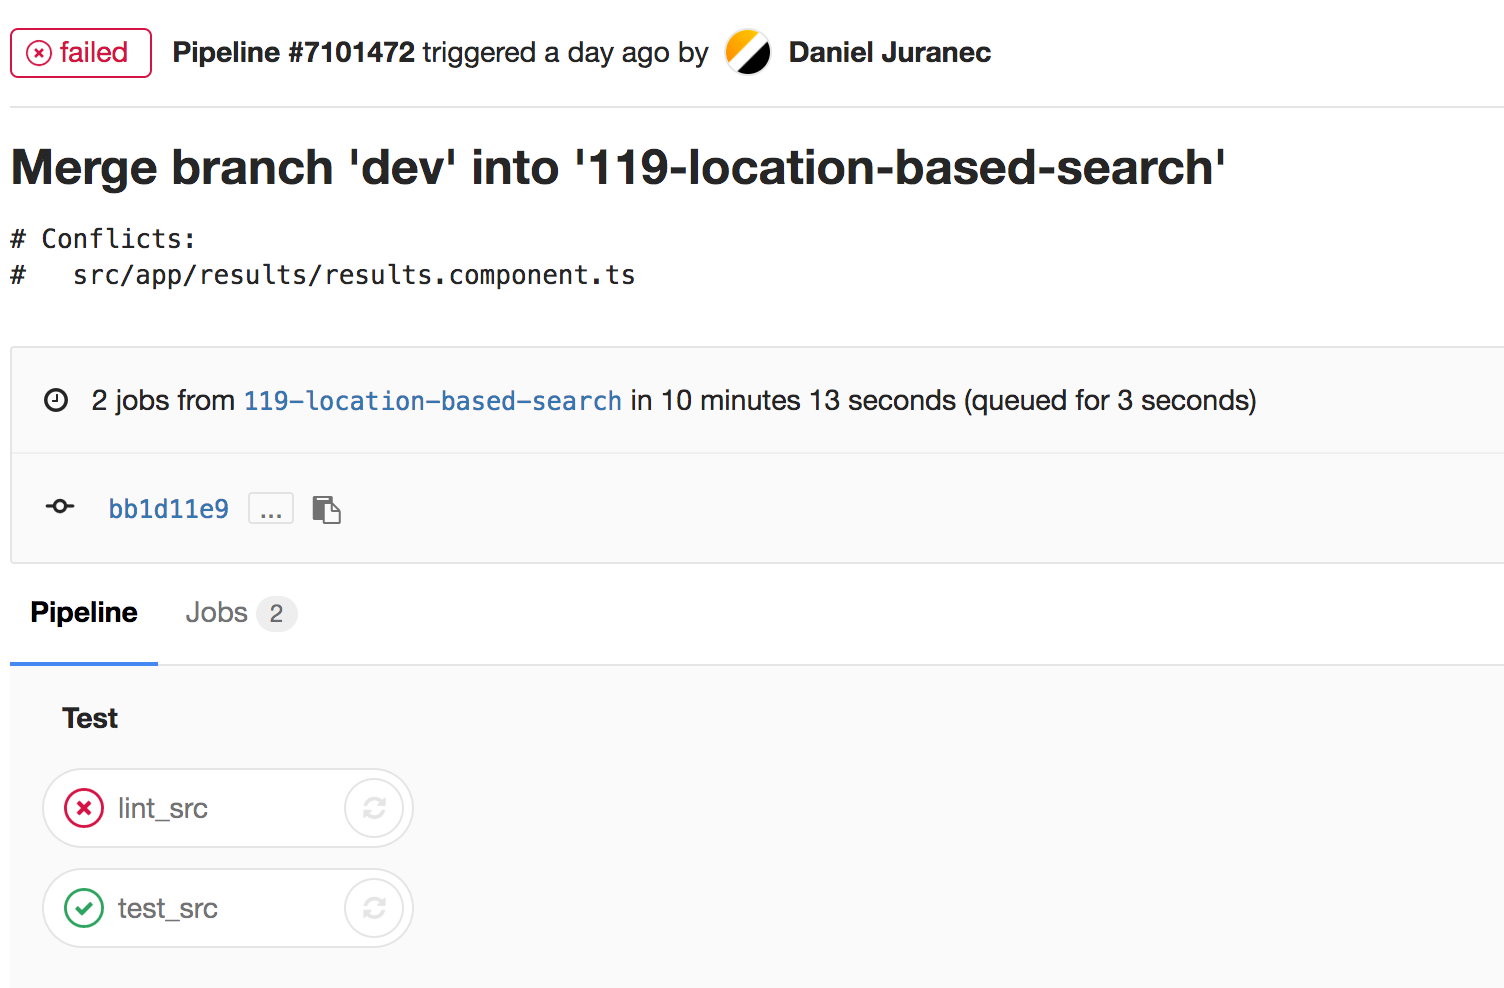
\includegraphics[width=9cm]{figures/cicd_failed_pipeline}
\end{center}
\caption{Example of a failed pipeline in GitLab}
\label{fig:cicd_failed_pipeline}
\end{figure}

 
% Considered combining test tasks
Merging these two tasks was considered, but left aside for now. The tasks take 5-10 minutes 
 each to run, and are run in parallel. The downside of this separation is the fact that \texttt{npm install} 
 is run twice. However, by leaving the tasks separate, we get a quicker, clearer indication
 of which part of the stage failed - actual functionality, or a style issue.

 \begin{figure}
\begin{center}
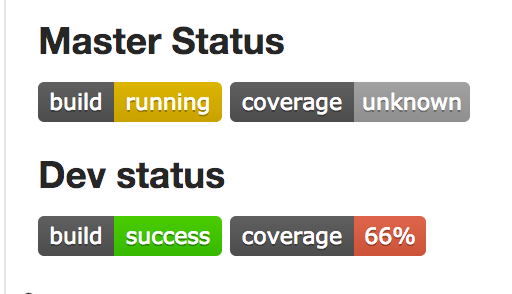
\includegraphics[width=4cm]{figures/cicd_coverage_buttons}
\end{center}
\caption{The buttons used to display pipeline status and test coverage}
\label{fig:cicd_coverage_buttons}
\end{figure}

% Describe deployment tasks
The Continuous deployment tasks were both essentially the same, but related to which branch was being 
 committed to. As both dev and master can only be merged into instead of committed to, these tasks can 
 be run only on merge commits to them. The tasks run tests (to allow coverage reports for the branches) 
 and then deploy to our live servers. The dev branch deploys to the staging zone, and 
 master to our production site. 
 
The fact that this is automated helps encourage rapid deployment, as the steps take some time, and are 
 boring for people to do. This methodology takes out the human steps, and means that the development team 
 can focus on development. These rapid deployments also help by making it easy for the team to demonstrate 
 and generate feedback from the public.


% consider how it helped us and how it could have been improved
The CI and CD processes helped us by keeping our code of high quality, preventing broken commits and reducing 
 manual time spent doing menial tasks. However, it took a fairly large period of time to get working and to
 optimise into time chunks that were consistent with the goal of 10 minutes. It is arguable that the time 
 could have been better spent working on the actual project itself. As a counterpoint to this, it could be
 argued that the CI and CD has saved the development team time in fixing bugs later on, and by ensuring code is more
 readable, reducing time wasted understanding the code.


%==============================================================================

\section{Conclusions}
\label{sec:conclusion}


Explain the wider lessons that you learned about software engineering,
based on the specific issues discussed in previous sections.  Reflect
on the extent to which these lessons could be generalised to other
types of software project.  Relate the wider lessons to others
reported in case studies in the software engineering literature.

%==============================================================================
\bibliographystyle{plain}
\bibliography{dissertation}
\end{document}
